% !TEX root =  centrtutorial.tex
%---------------------------------------------------------------------- SLIDE -

\frame{
  \frametitle{Roadmap}
  \begin{itemize}
    \item Introduction
      \begin{itemize}
        \item motivation, history, and definitions
        \item closeness and betweenness centrality
        \item axioms: what to look for in a centrality measure
      \end{itemize}
    \item Exact algorithms
      \begin{itemize}
        \item exact algorithms on static graphs
        \item exact algorithms on dynamic graphs
      \end{itemize}
    \item Approximation algorithms
      \begin{itemize}
        \item approximation algorithms on static graphs
        \item approximation algorithms on dynamic graphs
      \end{itemize}
    \item Conclusions
      \begin{itemize}
        \item open problems and research directions
      \end{itemize}
  \end{itemize}
}

\section{Introduction}

\frame{
  \frametitle{Social network analysis}
  \begin{itemize}
    \item Social network analysis is the study of social entities and their interactions and relationships.
      \pause \item The interactions and relationships can be represented with a network or graph,
      \begin{itemize}
        \pause  \item each vertex represents an actor
        \pause  \item each link represents a relationship
    \end{itemize}
    \pause \item From the graph, we can study the properties of its structure,
    and the \emph{role}, \emph{position}, and \emph{prestige} of each social entity.
    \pause\item We can also find various kinds of sub-graphs, e.g., \emph{communities} formed by groups of entities.
\end{itemize}
}

%---------------------------------------------------------------------- SLIDE -

\frame{
  \frametitle{Centrality in networks}
  \begin{itemize}
    \item Important or prominent actors are those that are linked or involved with other actors extensively
      \pause \item A person with extensive contacts (links) or communications with many other people in the organization is considered more important than a person with relatively fewer contacts
      \pause \item A central actor is one involved in many ties
      \pause \item \emph{Graph centrality} is a topic of uttermost importance in \emph{social sciences}
      \pause \item Also related to the problem of \emph{ranking} in the context of \emph{Web Search}:
      \begin{itemize}
        \item Each webpage is a social actor
        \item Each hyperlink is an endorsement relationship
        \item Centrality measures provide a query independent link-based score of \emph{importance} of a web page
      \end{itemize}
  \end{itemize}

}


%---------------------------------------------------------------------- SLIDE -

\frame{
  \frametitle{History of centrality (in a nutshell)}
  \begin{itemize}
    \pause\item first attempts in the late 1940s at M.I.T.~(Bavelas 1946), in the framework of communication patterns and
    group collaboration;
    \pause\item in the following decades, various measures of centralities were proposed and employed by social scientists in a myriad of contexts (Bavelas 1951; Katz 1953;
    Shaw 1954; Beauchamp 1965; Mackenzie 1966; Burgess 1969; Anthonisse 1971; Czapiel 1974...)
    \pause\item a new interest raised in the mid-90s with the advent of search engines: a ``reincarnation'' of centrality.
\end{itemize}


\pause Freeman (1979) observed:
\begin{quotation}
  ``several measures are often only vaguely related to
  the intuitive ideas they purport to index, and many are so complex that it is difficult
  or impossible to discover what, if anything, they are measuring''
\end{quotation}
}

%---------------------------------------------------------------------- SLIDE -

\frame{
  \frametitle{Types of centralities}
  Starting point: the central vertex of a star is the most important! Why?
  \begin{enumerate}
    \pause\item the vertex with largest degree;
    \pause\item the vertex that is closest to the other vertexes (e.g., that has the smallest average distance to other vertexes);
    \pause\item the vertex through which most shortest paths pass;
    \pause\item the vertex with the largest number of incoming paths of length $k$, for every $k$;
    \pause\item the vertex that maximizes the dominant eigenvector of the graph adjacency matrix;
    \pause\item the vertex with highest probability in the stationary distribution of the natural random walk on the graph.
\end{enumerate}
\pause These observations lead to corresponding competing views of centrality.
}

%---------------------------------------------------------------------- SLIDE -

\frame{
  \frametitle{Types of centralities}
  This observation leads to the following classes of indices of centrality:
  \begin{enumerate}
    \pause\item measures based on distances [degree, closeness, Lin's index];
    \pause\item measures based on paths [betweenness, Katz's index];
    \pause\item spectral measures [dominant eigenvector, Seeley's index, PageRank, HITS, SALSA].
\end{enumerate}

\medskip

\pause The last two classes  are largely the same,
(even if that wasn't fully understood for a long time).

}

%---------------------------------------------------------------------- SLIDE -
\frame{
  \frametitle{Geometric centralities}
  \begin{itemize}
    \pause\item \emph{degree} (folklore): $c_{\mathrm{deg}}(x)=d^-(x)$
    \pause\item \emph{closeness} (Bavelas, 1950):
    $c_{\mathrm{clos}}(x)=\closeness(x)=\frac1{\sum_y d(y,x)}$
    \pause\item \emph{Lin} (Lin, 1976):
    $c_{\mathrm{Lin}}(x)=\frac{r(x)^2}{\sum_y d(y,x)}$ where $r(x)$ is the
    number of vertexes that are co-reachable from $x$
    \pause\item \emph{harmonic} (Boldi, Vigna, 2013)
    $c_{\mathrm{harm}}(x)=\sum_{y\neq x}\frac1{d(y,x)}$
\end{itemize}
}

%---------------------------------------------------------------------- SLIDE -
\frame{
  \frametitle{Path-based centralities}
  \begin{itemize}
    \pause\item \emph{betweenness} (Anthonisse, 1971):
    $c_{\mathrm{bet}}(x)=\betw(x)=\sum_{y,z \neq x,\sigma_{yz}\neq 0}
    \frac{\sigma_{yz}(x)}{\sigma_{yz}}$ where $\sigma_{yz}$ is the number of
    shortest paths $y \to z$, and $\sigma_{yz}(x)$ is the number of such paths
    passing through $x$
    \pause\item \emph{Katz} (Katz, 1951):
    $c_{\mathrm{Katz}}(x)=\sum_{t\geq 0} \beta^t p_t(x)$ where $p_t(x)$ is the
    number of paths of length $t$ ending in $x$, and $\beta$ is a parameter
    ($\beta<1/\rho$)
\end{itemize}
}

%---------------------------------------------------------------------- SLIDE -
\frame{
  \frametitle{Spectral centralities}
  \begin{itemize}
    \item \emph{dominant} (Wei, 1953):
      $c_{\mathrm{dom}}(x)$ is the dominant (right) eigenvector of $G$
    \item \emph{Seeley} (Seeley, 1949):
      $c_{\mathrm{Seeley}}(x)$ is the dominant (left) eigenvector of $G_r$
    \item \emph{PageRank} (Brin, Page \emph{et al.}, 1999):
      $c_{\mathrm{PR}}(x)$ is the dominant (left) eigenvector of $\alpha
      G_r+(1-\alpha) \mathbf{1}^T\mathbf{1}/n$ (where $\alpha<1$)
    \item \emph{HITS} (Kleinberg, 1997):
      $c_{\mathrm{HITS}}(x)$ is the dominant (left) eigenvector of $G^TG$
    \item \emph{SALSA} (Lempel, Moran, 2001):
      $c_{\mathrm{SALSA}}(x)$ is the dominant (left) eigenvector of $G_c^TG_r$
  \end{itemize}

  \medskip

  {\small Where  $G$ denotes the adjacency matrix of the graph, $G_r$ is the the adjacency matrix normalized by row, and $G_c$ is the adjacency matrix normalized by column.}
}


%---------------------------------------------------------------------- SLIDE -
\subsection{Closeness and Betweenness}

%---------------------------------------------------------------------- SLIDE -
\frame{
  \frametitle{Closeness centrality}

  Motivation
  \begin{itemize}
    \item Measures the ability to quickly access or pass information through the graph
  \end{itemize}

  Definition:
  \begin{itemize}
    \item closeness centrality $\closeness(x)$ of a vertex $x$
      $$
      \closeness(x)=\frac{1}{\sum_{y \neq x \in V}d(y,x).}
      $$
      %\item \footnotesize
    \item $d(y,x)$ is the length of a shortest path between $y$ and $x$
    \item The closeness of a vertex is defined as the inverse of the sum of the shortest distances between the vertex and all other vertexes of the graph
  \end{itemize}
}



%---------------------------------------------------------------------- SLIDE -
\frame{
  \frametitle{Betweenness centrality}
  Motivation
  \begin{itemize}
    \item Measures the frequency with which a user appears in a shortest
      path between two other users
  \end{itemize}

  \begin{columns}[T]
    \begin{column}{55mm}
      Definition:
      \begin{itemize}
        \item  betweenness centrality $\betw(x)$ of a vertex $x$:
          \[
            \betw(x)=\sum_{\substack{s\neq x\neq t \in V\\s\neq t}}
            \frac{\sigma_{st}(x)}{\sigma_{st}}
          \]
        \item[\footnotesize $\sigma_{st}$]:  number of different shortest paths
          between vertexes $s$ \& $t$
        \item[\footnotesize $\sigma_{st}(x)$:] how many of them pass through vertex $x$
      \end{itemize}
    \end{column}
    \begin{column}{45mm}
      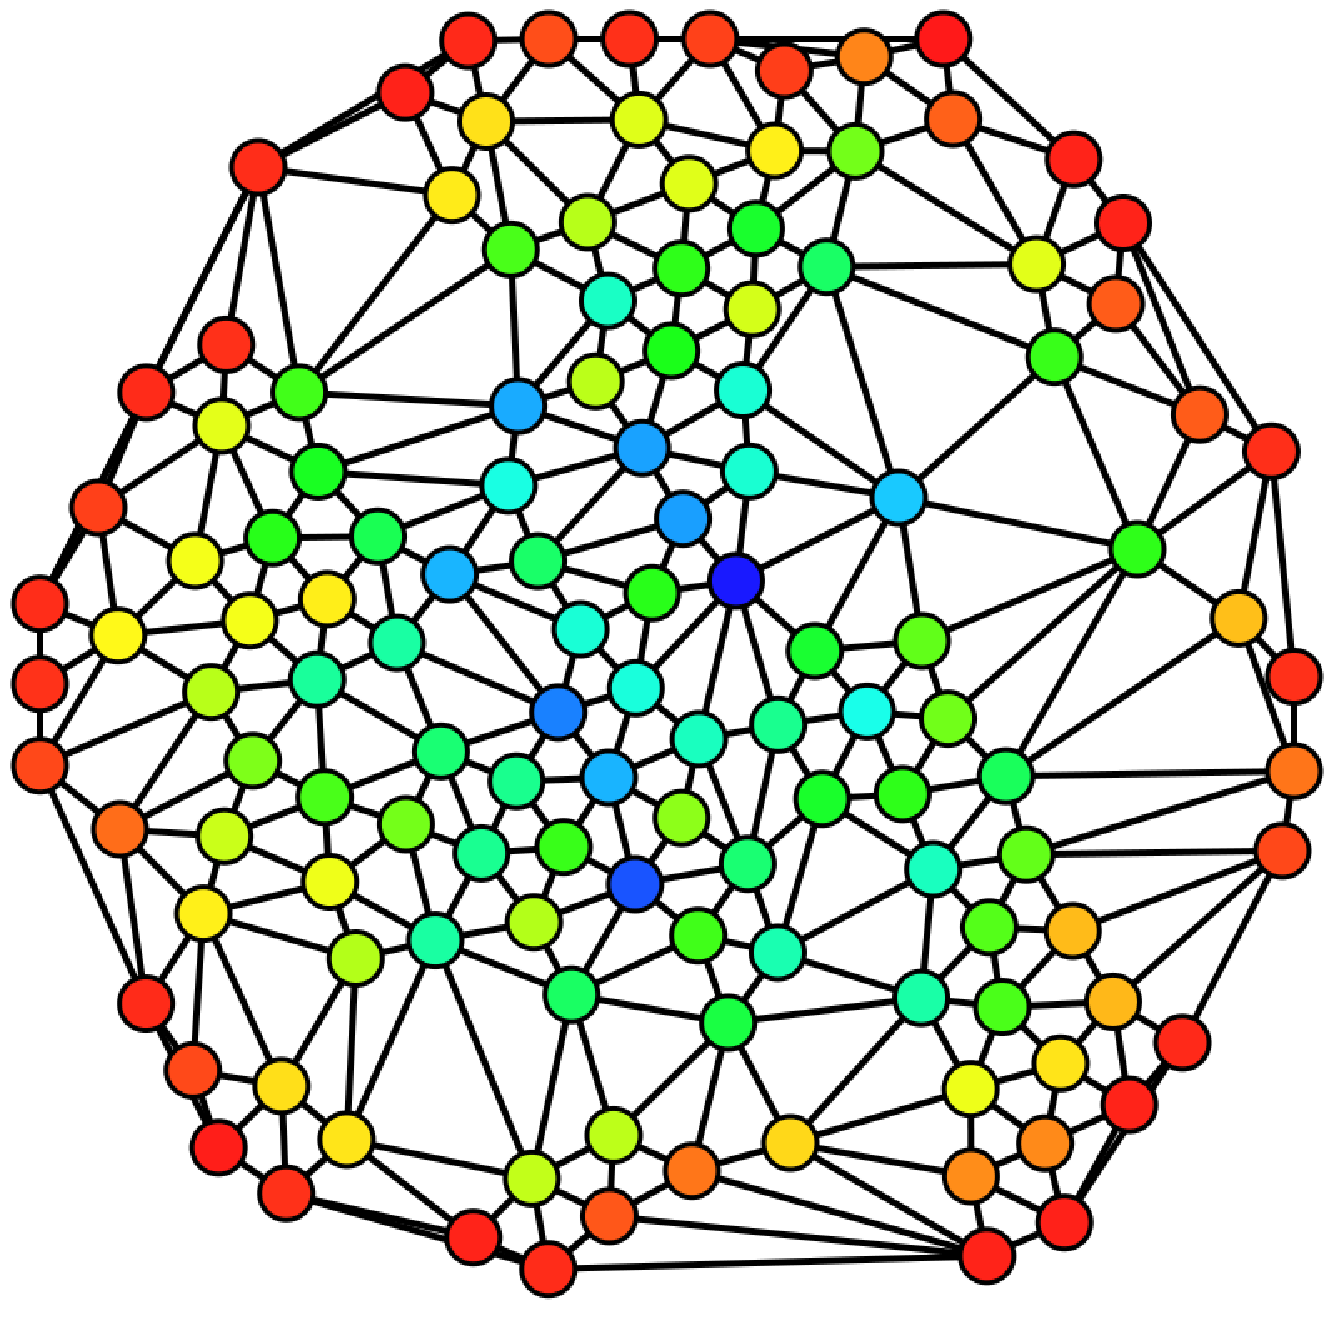
\includegraphics[width=42mm]{imgs/Graph_betweenness.pdf}
      \\ \hspace{10mm} \tiny{Example retrieved from  Wikipedia}
    \end{column}
  \end{columns}
}

%---------------------------------------------------------------------- SLIDE -
\frame{
  \frametitle{Betweenness centrality}
  \begin{itemize}
    \item Can be defined also for edges (similarly to vertexes)
    \item Edges with high betweenness are what sociologists call \emph{``weak ties''}
    \item They tend to be the \emph{bridge} between two communities
  \end{itemize}

  \begin{columns}[T]
    \begin{column}{60mm}
      \emph{The strength of weak ties (Granovetter 1973)}
      \begin{small}
        \begin{itemize}
          \item Dissemination and coordination dynamics are influenced by links established to vertexes of different communities.
          \item The importance of these links has become more and more with the rise of social networks and professional networking platforms.
        \end{itemize}
      \end{small}
    \end{column}
    \hspace{-16mm}\begin{column}{40mm}
      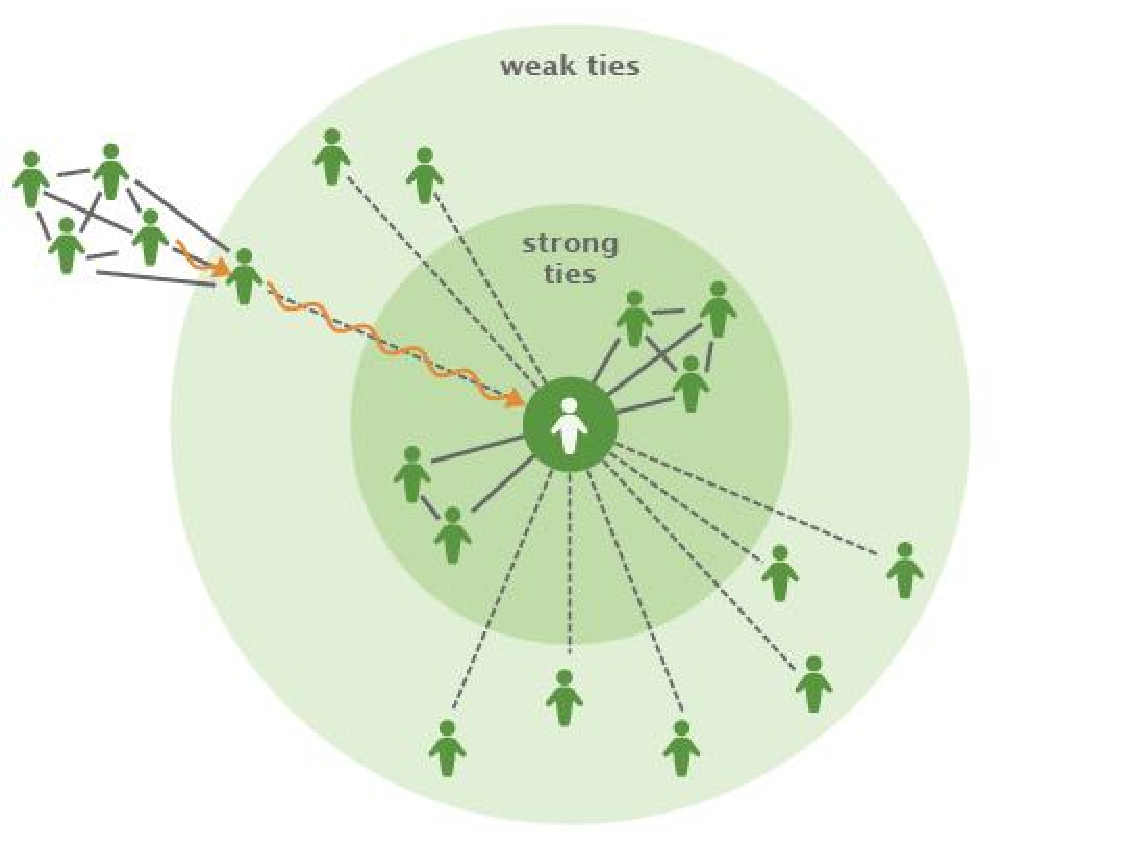
\includegraphics[width=62mm]{imgs/weak_ties.pdf}
    \end{column}
  \end{columns}
}

%---------------------------------------------------------------------- SLIDE -
\frame{
  \frametitle{Weak ties}
  (Bakshy et al. 2012)
  \begin{itemize}
    \item
      Weak links have a greater potential to expose links to new  contacts that otherwise would not have been discovered.
  \end{itemize}

  \begin{center}
    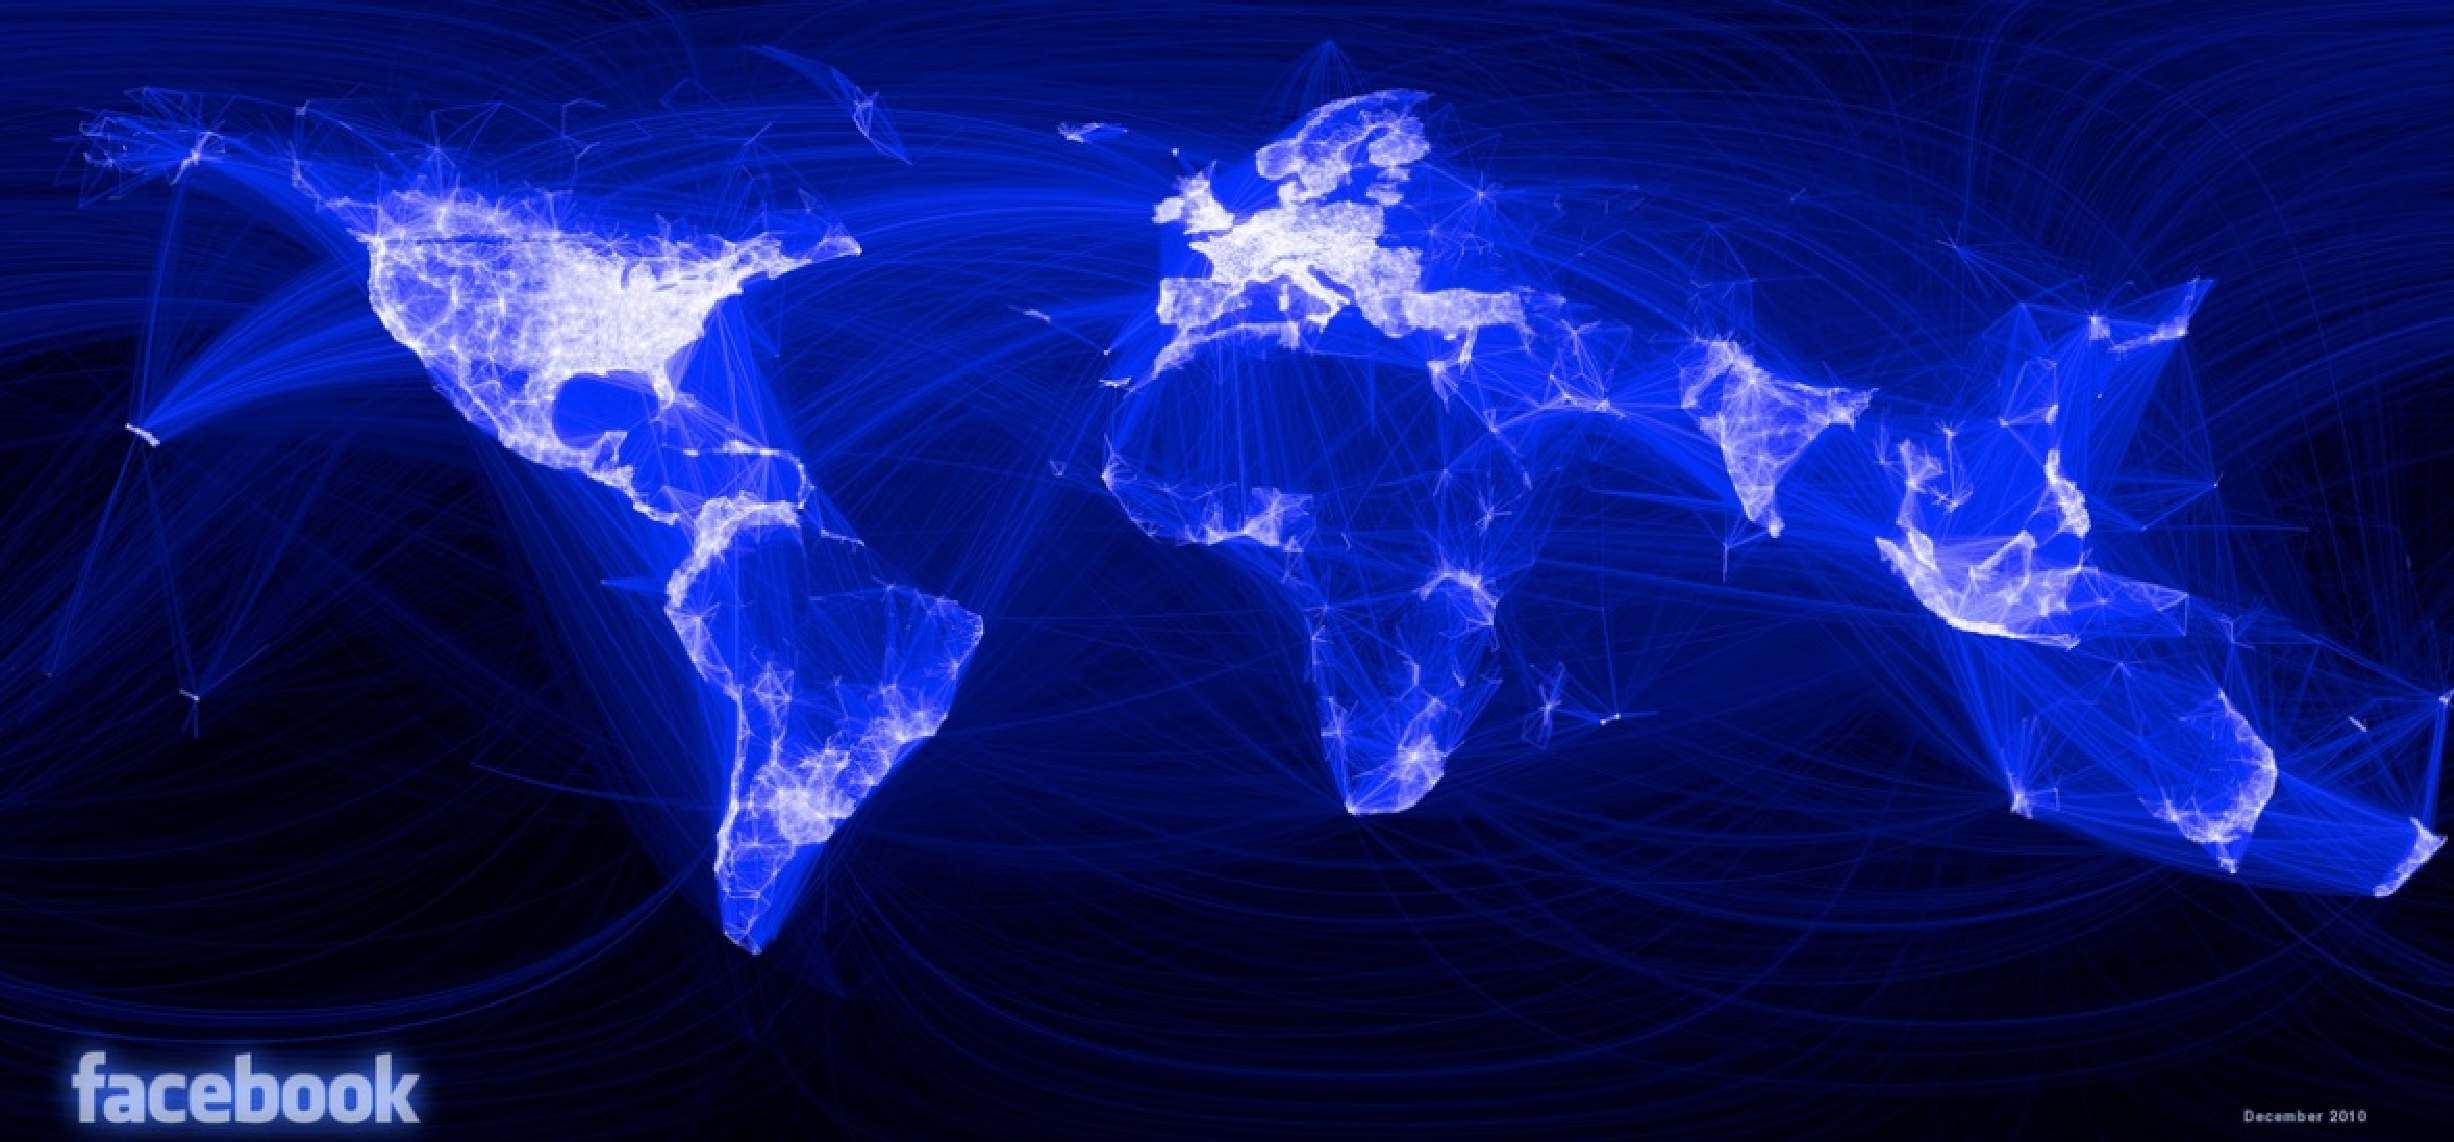
\includegraphics[width=70mm]{imgs/facebook_graph.pdf}
  \end{center}
}

%---------------------------------------------------------------------- SLIDE -
\frame{
  \frametitle{Weak ties}
  (Grabowicz et al. 2012)
  \begin{itemize}
    \item Personal interactions are more likely to occur in internal links within communities (strong links)
    \item Events or new information is propagated faster by intermediate links (weak links).
  \end{itemize}

  \medskip

  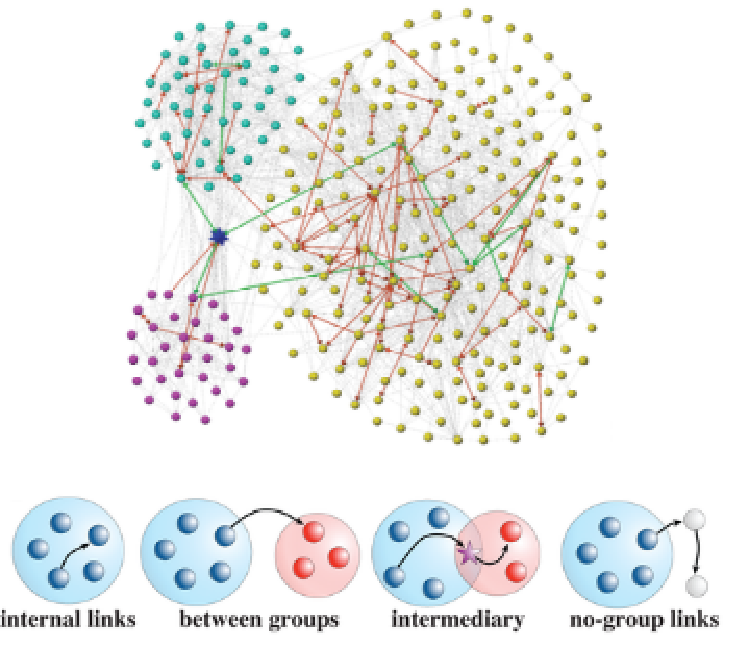
\includegraphics[width=50mm]{imgs/weak_ties2.pdf}
  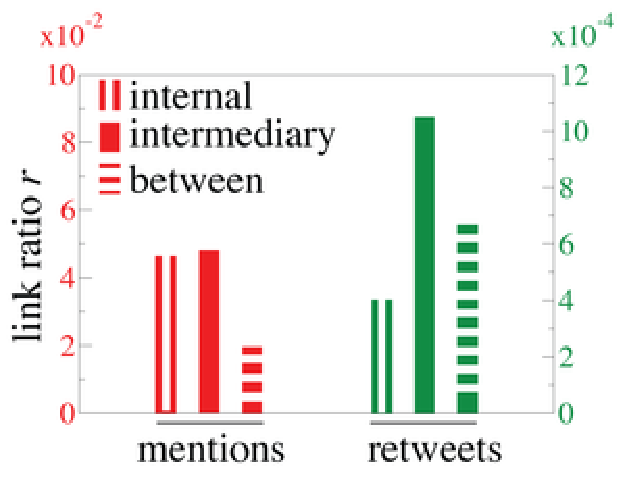
\includegraphics[width=50mm]{imgs/weak_ties3.pdf}
}

%---------------------------------------------------------------------- SLIDE -
\frame{
  \frametitle{Girvan-Newman algorithm for community detection (Girvan and Newman 2002)}
  Hierarchical divisive clustering obtained by \emph{recursively removing the ``weakest tie''}.

  \begin{enumerate}
    \item Compute edge betweenness centrality of all edges;
    \item Remove the edge with the highest betweenness centrality;
    \item Repeat from 1.
  \end{enumerate}

  \medskip
  \centering
  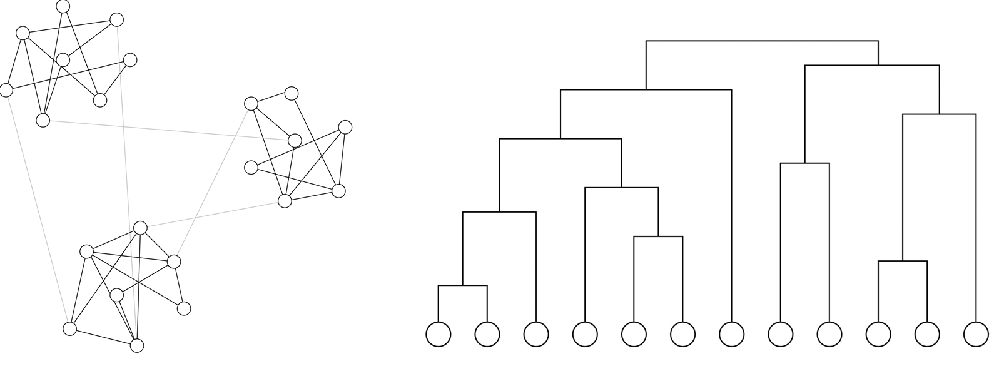
\includegraphics[width=82mm]{imgs/gn.pdf}
}




%---------------------------------------------------------------------- SLIDE -
\frame{
  \frametitle{Comparison}
  \begin{block}{Which vertex is the most central?}
    \begin{itemize}
      \item for Degree Centrality:
      \item for Closeness Centrality:
      \item for Betweenness Centrality:
    \end{itemize}
  \end{block}
  \centering
  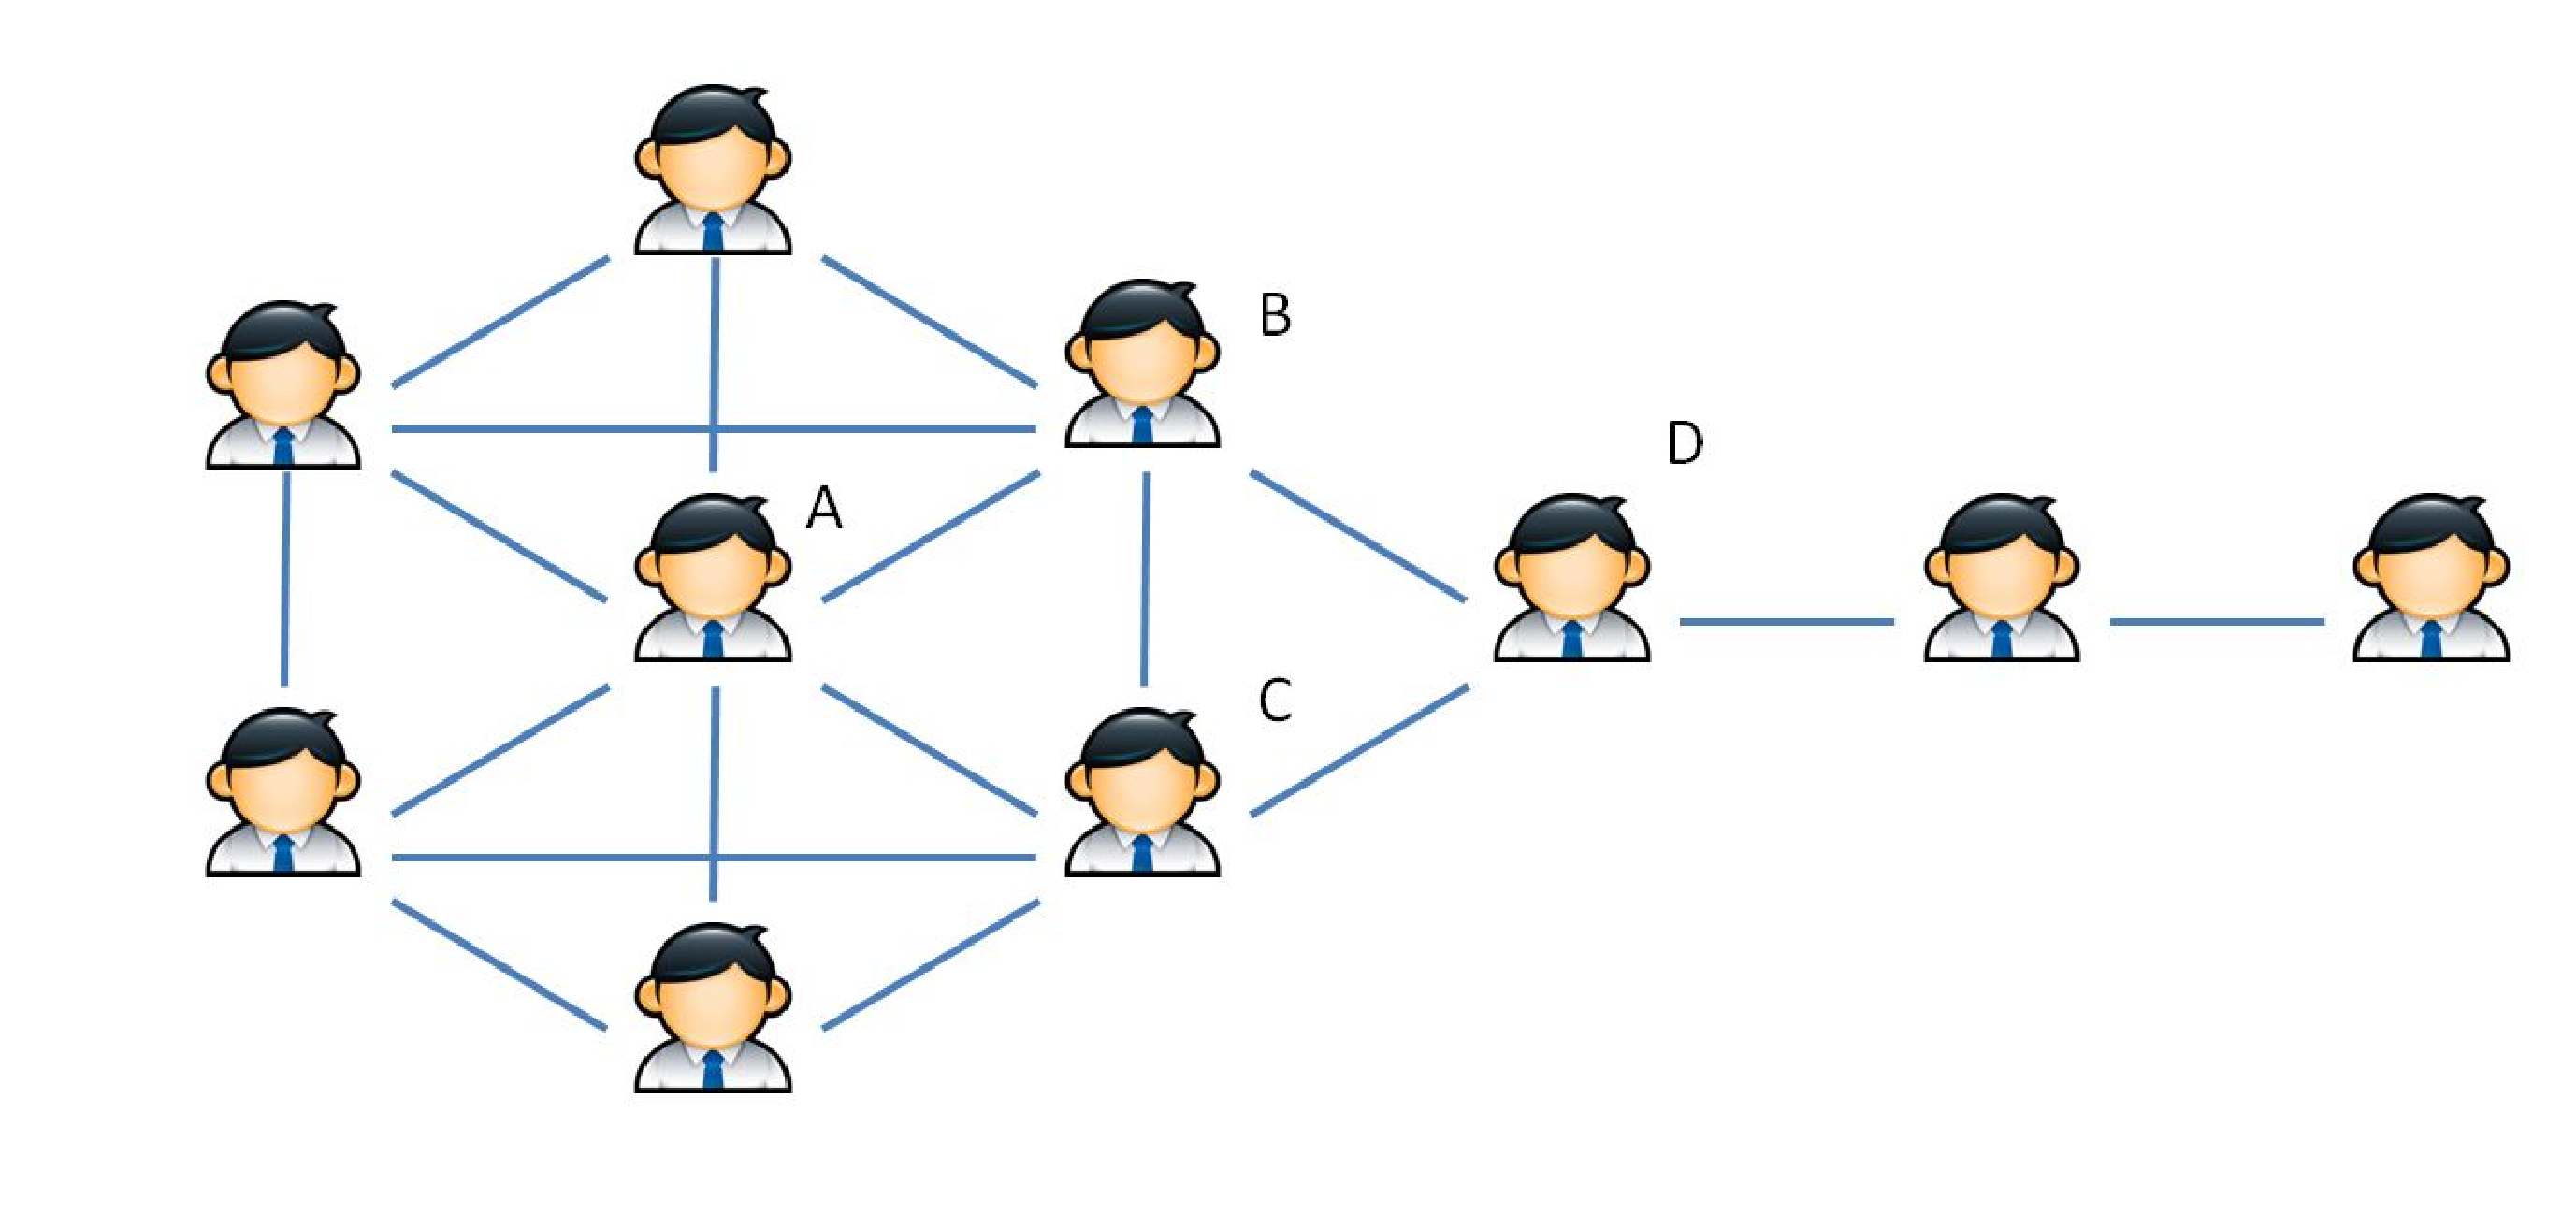
\includegraphics[width=100mm]{imgs/centrality_comparison.pdf}
}

\frame{
  \frametitle{Comparison}
  \begin{block}{Which vertex is the most central?}
    \begin{itemize}
      \item for Degree Centrality:  {\color{blue}  user A}
      \item for Closeness Centrality:
      \item for Betweenness Centrality:
    \end{itemize}
  \end{block}
  \centering
  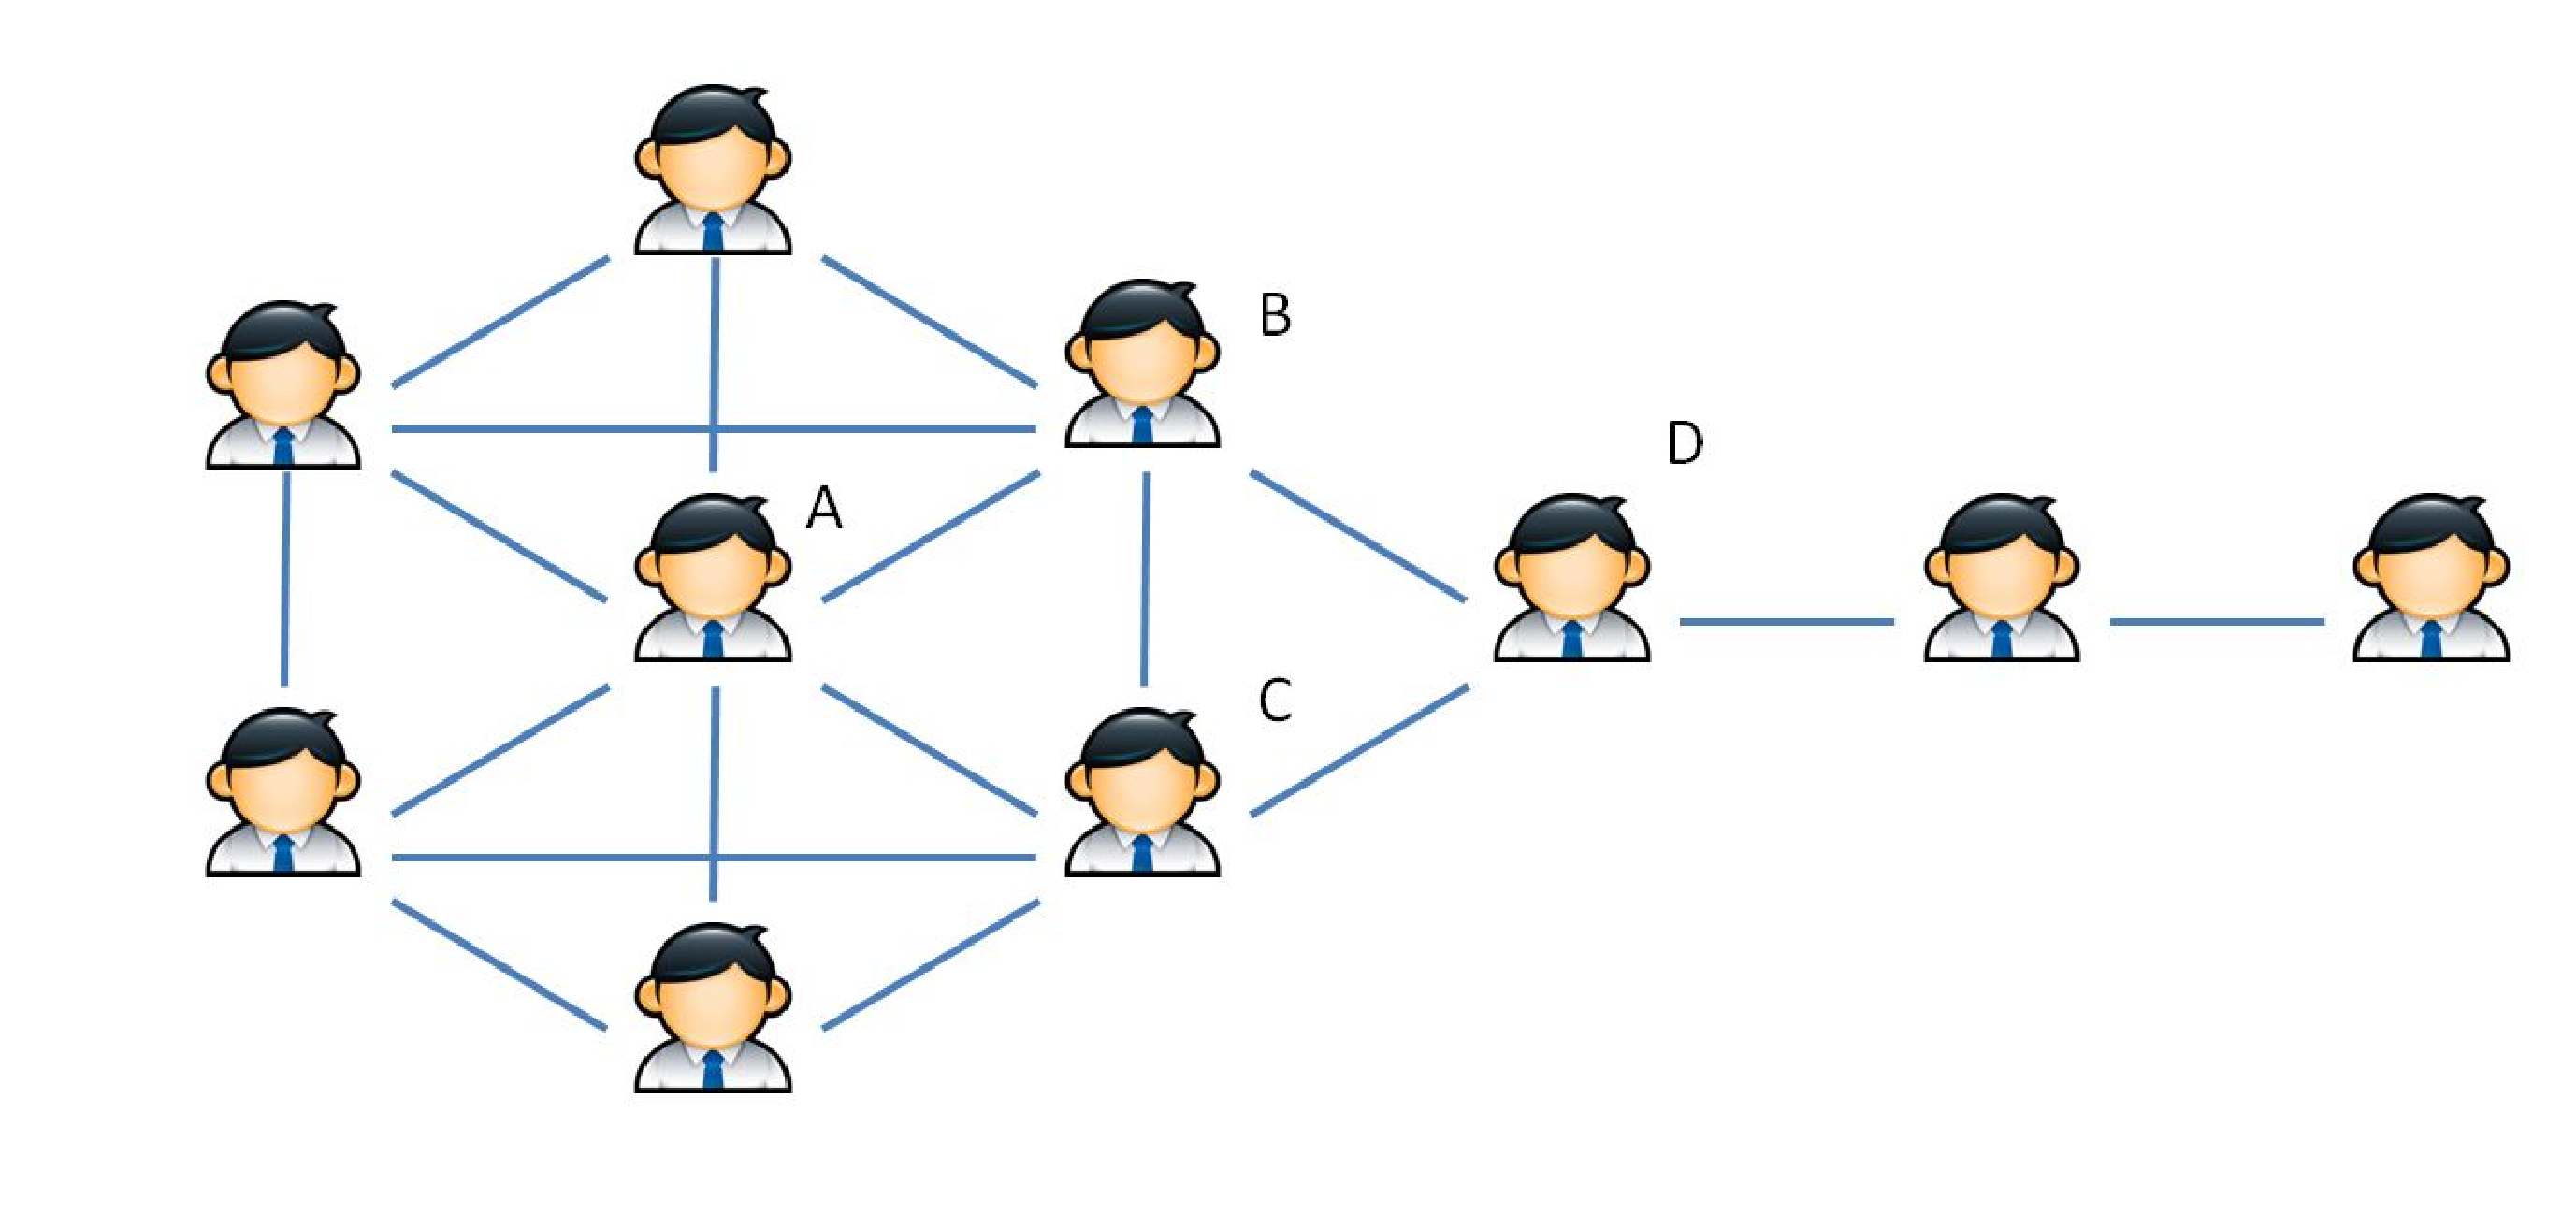
\includegraphics[width=100mm]{imgs/centrality_comparison.pdf}
}

\frame{
  \frametitle{Comparison}
  \begin{block}{Which vertex is the most central?}
    \begin{itemize}
      \item for Degree Centrality: {\color{blue}  user A}
      \item for Closeness Centrality: {\color{blue}  users B and C}
      \item for Betweenness Centrality:
    \end{itemize}
  \end{block}
  \centering
  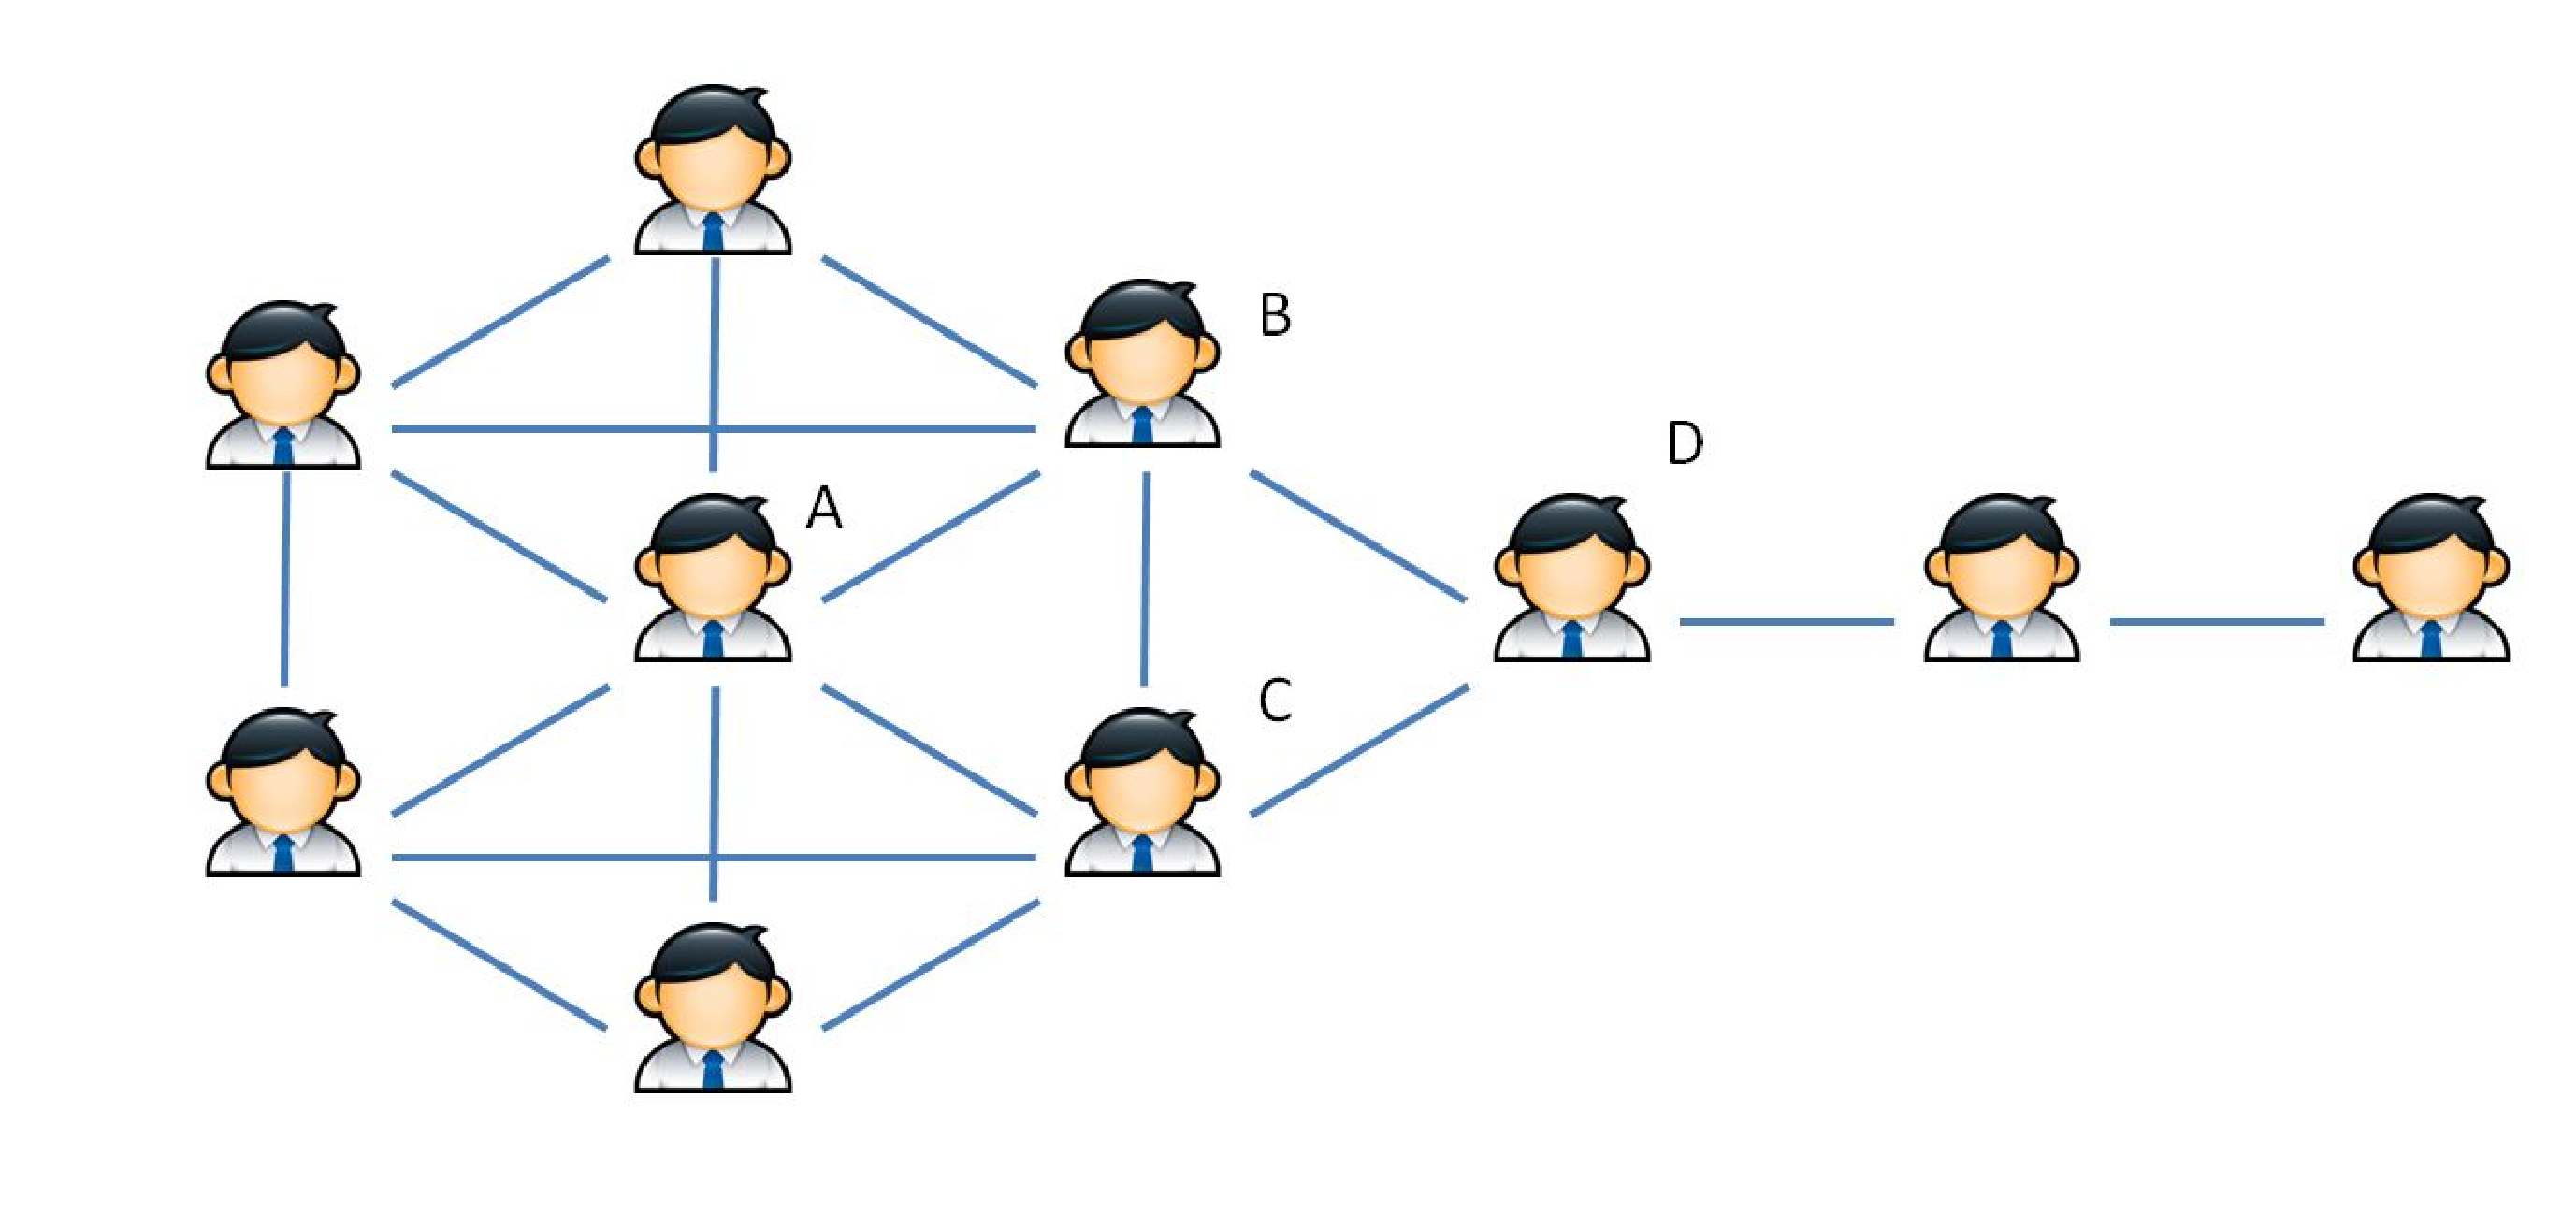
\includegraphics[width=100mm]{imgs/centrality_comparison.pdf}
}

\frame{
  \frametitle{Comparison}
  \begin{block}{Which vertex is the most central?}
    \begin{itemize}
      \item for Degree Centrality: {\color{blue}  user A}
      \item for Closeness Centrality: {\color{blue}  users B and C}
      \item for Betweenness Centrality: {\color{blue}  user D}
    \end{itemize}
  \end{block}
  \centering
  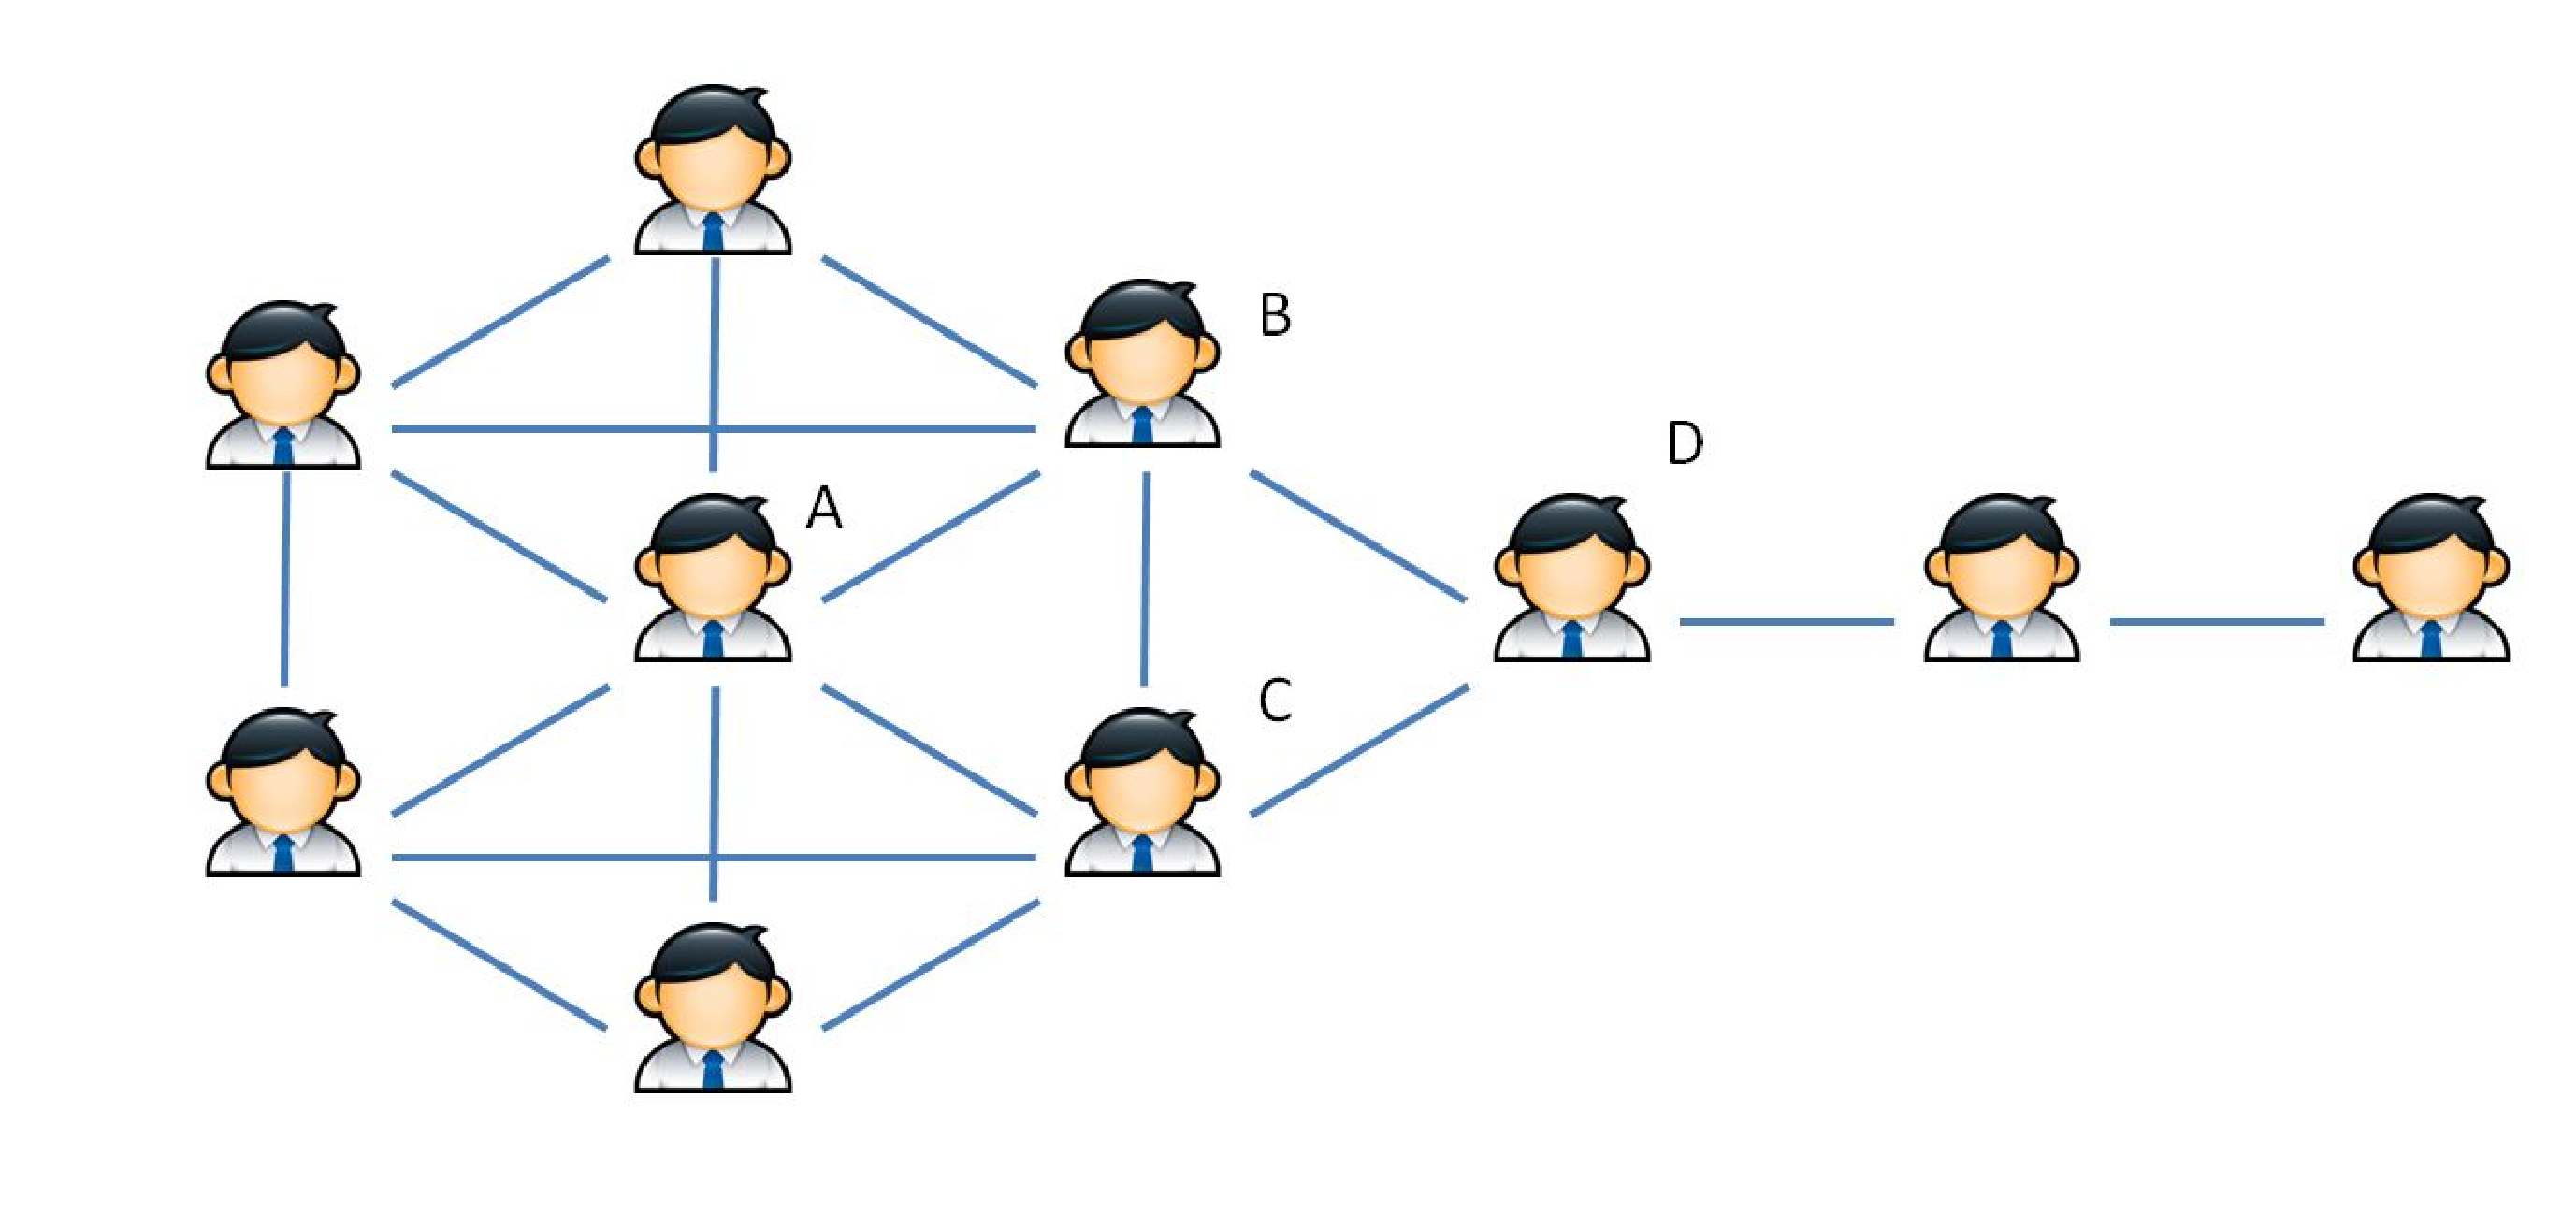
\includegraphics[width=100mm]{imgs/centrality_comparison.pdf}
}

%---------------------------------------------------------------------- SLIDE -
\frame{
  \frametitle{Visual Comparison}
  \begin{itemize}
    \item[A] Degree Centrality
    \item[B] Closeness Centrality
    \item[C] Betweenness Centrality
  \end{itemize}

  \centering
  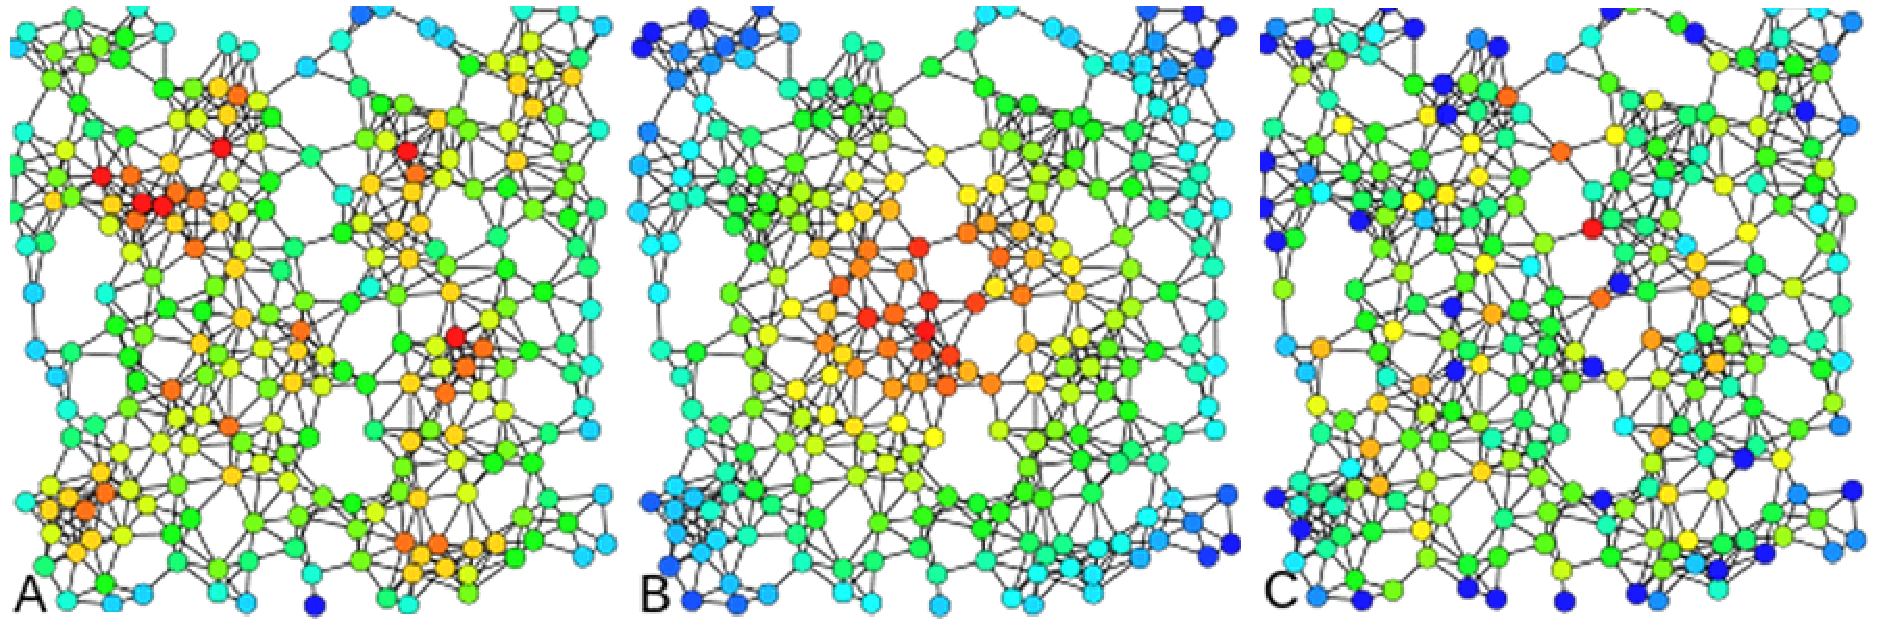
\includegraphics[width=100mm]{imgs/centrality.pdf}
}




%---------------------------------------------------------------------- SLIDE -
\subsection{Axioms for centrality (Boldi and Vigna 2013)}




%---------------------------------------------------------------------- SLIDE -
\frame{
  \frametitle{Assessing}
  Is there a robust way to convince oneself that a certain centrality measure is
  better than another?

  Axiomatization\dots
  \begin{itemize}
    \pause\item \dots hard axioms (characterize a centrality measure completely)
    \pause\item \dots soft axioms (like the $T_i$ axioms for topological spaces)
\end{itemize}
}

%---------------------------------------------------------------------- SLIDE -
\frame{
  \frametitle{Sensitivity to size}
  Idea: size matters!

  $S_{k,p}$ be the union of a $k$-clique and a $p$-cycle.
  \begin{itemize}
    \item if $k\to\infty$, every vertex of the clique becomes ultimately
      strictly more important than every vertex of the cycle
    \item if $p\to\infty$, every vertex of the cycle becomes ultimately
      strictly more important than every vertex of the clique
  \end{itemize}

  \medskip
  \centering
  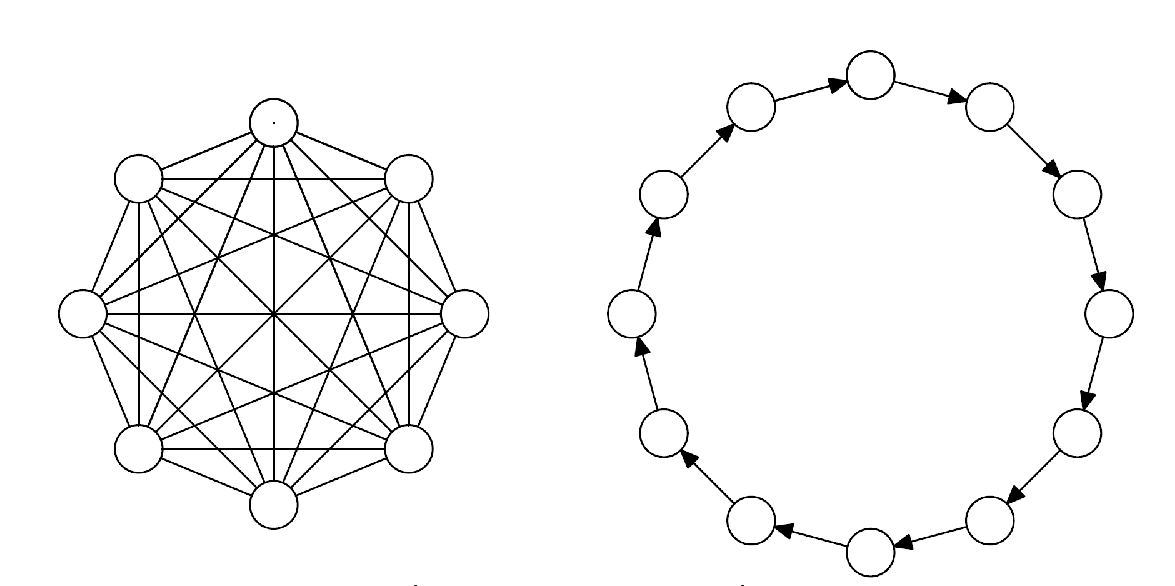
\includegraphics[width=82mm]{imgs/sts.pdf}
}

%---------------------------------------------------------------------- SLIDE -
\frame{
  \frametitle{Sensitivity to density}
  Idea: density matters!

  $D_{k,p}$ be made by a $k$-clique and a $p$-cycle connected by a single
  bidirectional bridge:
  \begin{itemize}
    \item if $k\to\infty$, the vertex on the clique-side of the bridge
      becomes more important than the vertex on the cycle-side.
  \end{itemize}

  \medskip
  \centering
  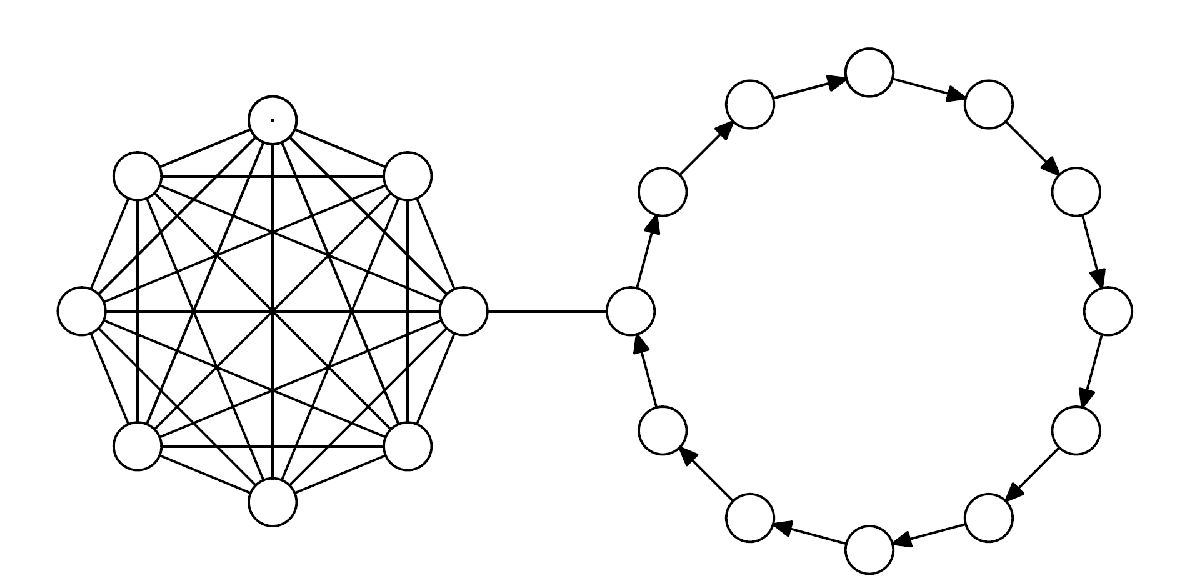
\includegraphics[width=82mm]{imgs/std.pdf}
}

%---------------------------------------------------------------------- SLIDE -
\frame{
  \frametitle{Score monotonicity}
  Adding an edge $x \to y$ strictly increases the score of $y$.

  \smallskip
  \pause {\bf Doesn't say anything about the score of other vertexes!}
}

%---------------------------------------------------------------------- SLIDE -
\frame{
  \frametitle{Rank monotonicity}
  Adding an edge $x \to y$\dots
  \begin{itemize}
    \pause\item if $y$ used to dominate $z$, then the same holds after adding
    the edge
    \pause\item if $y$ had the same score as $z$, then the same holds after
    adding the edge
    \pause\item {\bf strict variant: } if $y$ had the same score as $z$, then $y$
    dominates $z$ after adding the edge
\end{itemize}
}

%---------------------------------------------------------------------- SLIDE -
\frame{
  \frametitle{Rank monotonicity}
  \begin{table}
    \renewcommand{\arraystretch}{1.2}
    \begin{minipage}{\textwidth}
      \centering
      \begin{tabular}{l|c|c|c|c|c|c}
        \multicolumn{1}{c|}{}&\multicolumn{4}{c|}{Monotonicity}&\multicolumn{2}{c}{Other axioms}\\
        \multicolumn{1}{c|}{}&\multicolumn{2}{c|}{General}&\multicolumn{2}{c|}{Strongly connected}&\multicolumn{2}{c}{}\\
        Centrality & Score & Rank & Score & Rank & Size & Density
        \\
        \hline
        Harmonic & yes  & yes* & yes & yes* & yes & yes \\
        Degree  & yes & yes* & yes & yes* & only $k$ & yes \\
        Katz & yes & yes*& yes & yes* & only $k$ & yes \\
        PageRank &  yes & yes*& yes & yes* & no & yes \\
        Seeley & no & no & yes & yes & no & yes \\
        Closeness & no  & no & yes & yes & no & no \\
        Lin & no & no & yes & yes & only $k$& no \\
        Betweenness & no & no & no & no & only $p$ & no \\
        Dominant & no & no &? &? & only $k$ & yes \\
        HITS & no & no & no &no & only $k$ &yes\\
        SALSA & no & no & no &no & no & yes
      \end{tabular}
    \end{minipage}
  \end{table}
}

%---------------------------------------------------------------------- SLIDE -
\frame{
  \frametitle{Kendall's $\tau$}

  \begin{tabular}{c}
    Hollywood collaboration network\\
    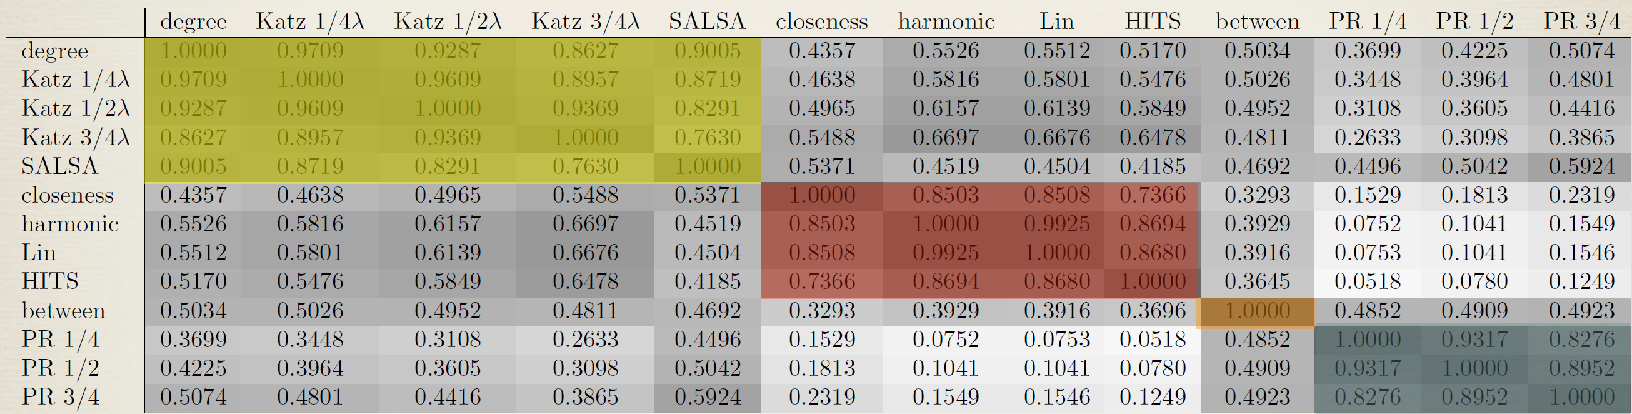
\includegraphics[width=\textwidth]{imgs/kendall2.pdf}\\
    \medskip \\
    .uk (May 2007 snapshot)\\
    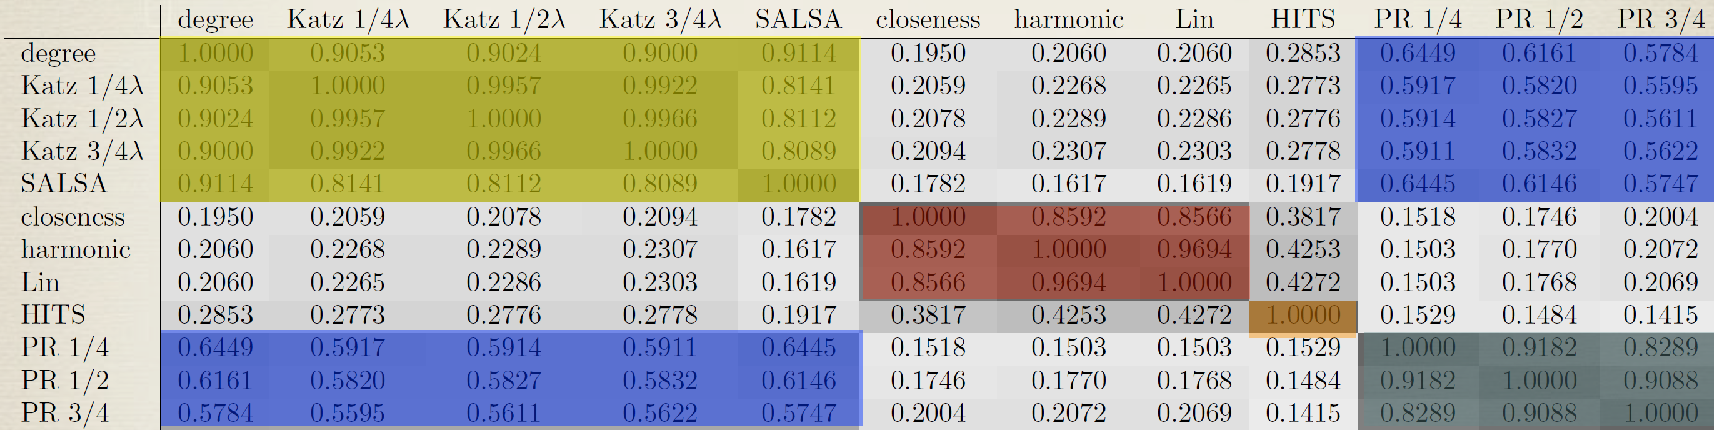
\includegraphics[width=\textwidth]{imgs/kendal.pdf}\\
  \end{tabular}
}

%---------------------------------------------------------------------- SLIDE -
\frame{
  \frametitle{Correlation}
  \begin{itemize}
    \pause \item most geometric indices and HITS
    are rather correlated to one another;
    \pause \item Katz, degree and SALSA are also
    highly correlated;
    \pause \item PageRank stands alone in the first dataset, but it is correlated to degree, Katz, and SALSA in the second dataset;
    \pause \item Betweenness is not correlated to anything in the first dataset, and could not be computed in the second dataset due to the size of the graph (106M vertices).
\end{itemize}

}
